\subsubsection{Monitor} \mbox{} \vspace{1pt}

La manera en que controlamos la ocupación de los espacios en el mapa, es decir, cómo evoluciona la trayectoria de cada robot es mediante el disparo de un Monitor implementado en Python. Este es el va a controlar, guiar y realizar la toma de decisiones para que cada robot pueda seguir su trayectoria sin interrumpir a los demás y por lo tanto no bloquear todo el sistema.

Para poder guiar a cada robot en su trayectoria, cada uno va a estar representado por un hilo lógico en el programa en Python. Más precisamente cuando existe un robot en el mundo real y se realiza el proceso de sincronización con el software, este va a crear un objeto (representación de un ente en la Programación Orientada a Objetos) el cual va a contener un conjunto de métodos implementados y entre ellos, la creación de un hilo en Python.

A su vez definimos cuál va a ser el punto de inicio y el punto final, es decir el comienzo del recorrido y el final del mismo, y el mapa es un modelo discreto representado por una Red de Petri. Podemos determinar cuales van a ser la plazas que el robot va a ocupar en un preciso momento y las transiciones que se van a disparar para que este pueda llegar a su destino. Con todos estos elementos le damos al monitor las herramientas para realizar su trabajo y efectuar los métodos que le permitan modificar el marcado de la Red de Petri.

\paragraph{Cola de cortesía} \mbox{} \vspace{5pt}

La manera en que el Monitor ejerce el control de la exclusión mutua dentro de la Red de Petri es mediante el uso de colas, entonces, cuando un hilo (robot) está dentro del monitor y aparece otro hilo que intenta ejecutar otro o el mismo procedimiento, el acceso al Monitor se bloquea e inserta el segundo hilo en una cola de cortesía usando una política FIFO. Cuando el primer hilo abandona el monitor, el segundo hilo (que se encuentra en el primer lugar de la cola) es el seleccionado por el Monitor para ejecutar sus tareas. Si la cola está vacía entonces el Monitor se encuentra libre y cualquier hilo que intente tomar el control de éste último podrá hacerlo sin intervención alguna.

\paragraph{Políticas} \mbox{} \vspace{5pt}

Así como mencionamos más arriba que hacemos uso de las colas del monitor para controlar la exclusión mutua, existe la posibilidad de que dos hilos (robots) intenten acceder a la misma plaza ya que su secuencia de disparos así lo determina. En ese caso vamos a tener que tomar una decisión de qué hilo es que va a lograr apoderarse de la plaza en primer lugar. Para esto hacemos uso de una Política definida por nosotros mismos, a partir de ella un hilo va a tener preferencia sobre otro.

Poniendo el caso en concreto de los robots que comparten un mapa, nos parece más acertada la idea de que un robot pueda terminar su recorrido de forma rápida y efectiva. Es por ello que cada robot va guardando el camino que va atravesando, es decir, las celdas por las cuales se desplazó y aumentando un contador interno. Este es el parámetro que se usa para determinar qué robot va a tener preferencia sobre otro, entonces, al momento de ocurrir un conflicto entre dos robots que intentan ocupar la misma celda, el Monitor va a evaluar que robot es el que tiene un mayor camino recorrido y elegirlo para ocupar el lugar en disputa.

\paragraph{Solución de conflictos entre robots} \mbox{} \vspace{5pt}

Acá representamos el posible conflicto que puede ocurrir cuando dos robots intentan ocupar el mismo lugar, como se representan en el mapa y su traducción en una Red de Petri.

\begin{figure}[H]
    \centering
    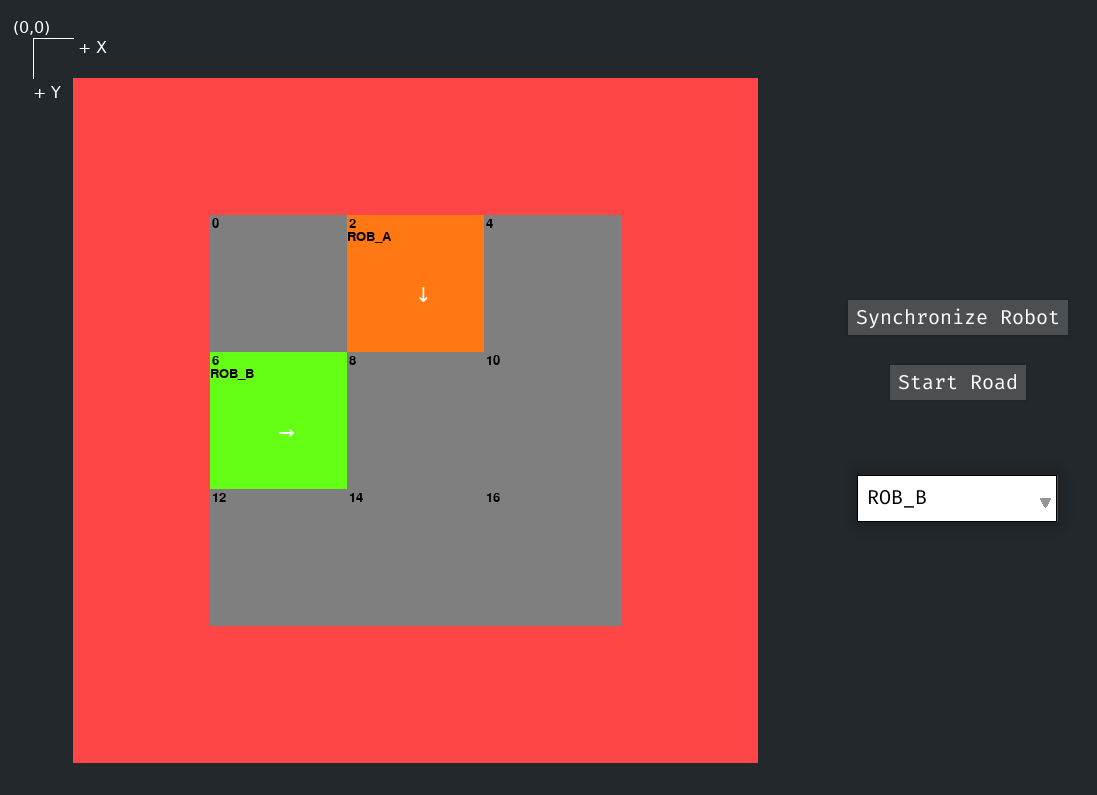
\includegraphics[width=0.7\linewidth]{images/conflicto_map.png}
    \caption{Representación de un conflicto entre dos robots que intentan pasar por la misma celda}
    \label{fig:conflicto_map}
\end{figure}

\begin{figure}[H]
    \centering
    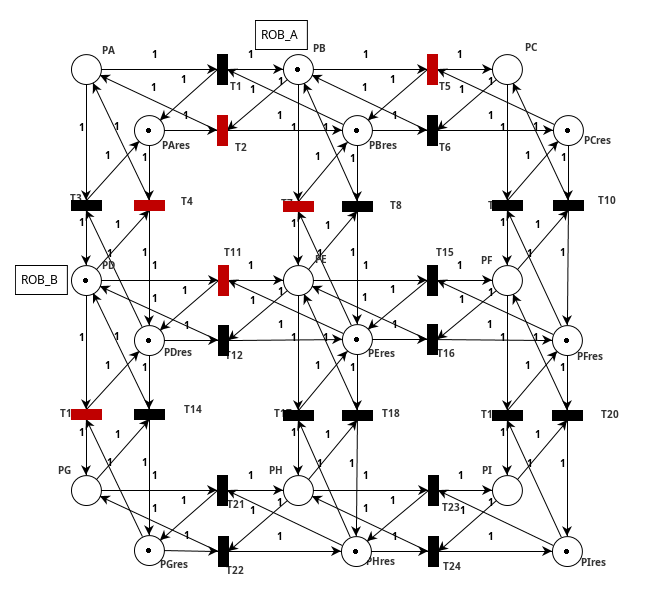
\includegraphics[width=0.7\linewidth]{images/rdp_no_grid_conflicto.png}
    \caption{Representación del conflicto de la figura \ref{fig:conflicto_map} en una red de Petri}
    \label{fig:rdp_no_grid_conflicto}
\end{figure}

\begin{figure}[H]
    \centering
    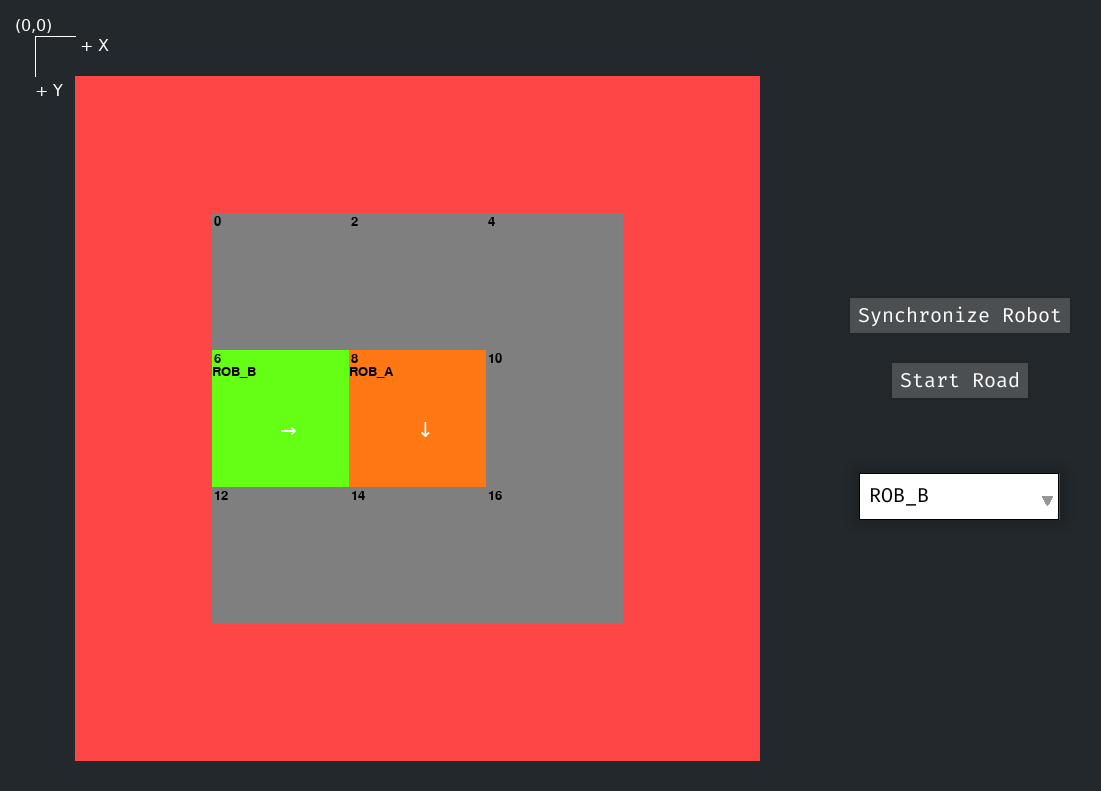
\includegraphics[width=0.7\linewidth]{images/conflicto_map_solucionado.png}
    \caption{Resolución del conflicto de dos robots intentando pasar por la misma celda}
    \label{fig:conflicto_map_solucionado}
\end{figure}

\begin{figure}[H]
    \centering
    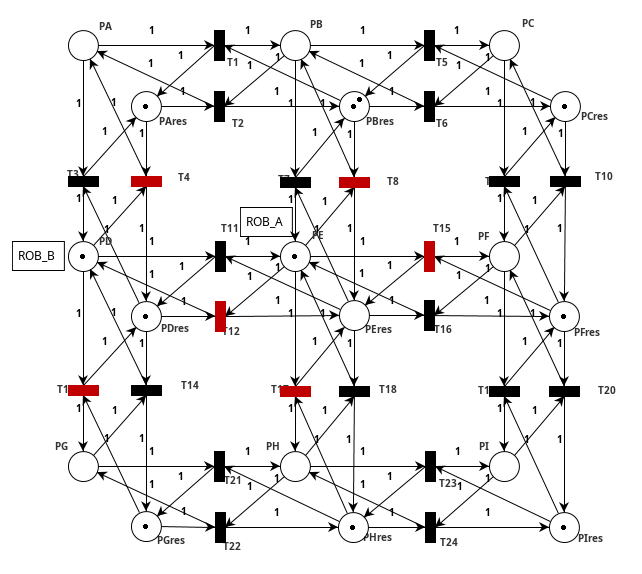
\includegraphics[width=0.7\linewidth]{images/rdp_no_grid_conflicto_solucionado.png}
    \caption{Resolución del conflicto entre los robots representado en una red de Petri y con el nuevo marcado de la red}
    \label{fig:rdp_no_grid_conflicto_solucionado}
\end{figure}

\paragraph{Funcionamiento del monitor} \mbox{} \vspace{10pt}

El funcionamiento del módulo del Monitor en Python queda representado en el siguiente Diagrama de secuencia.

\begin{figure}[H]
    \centering
    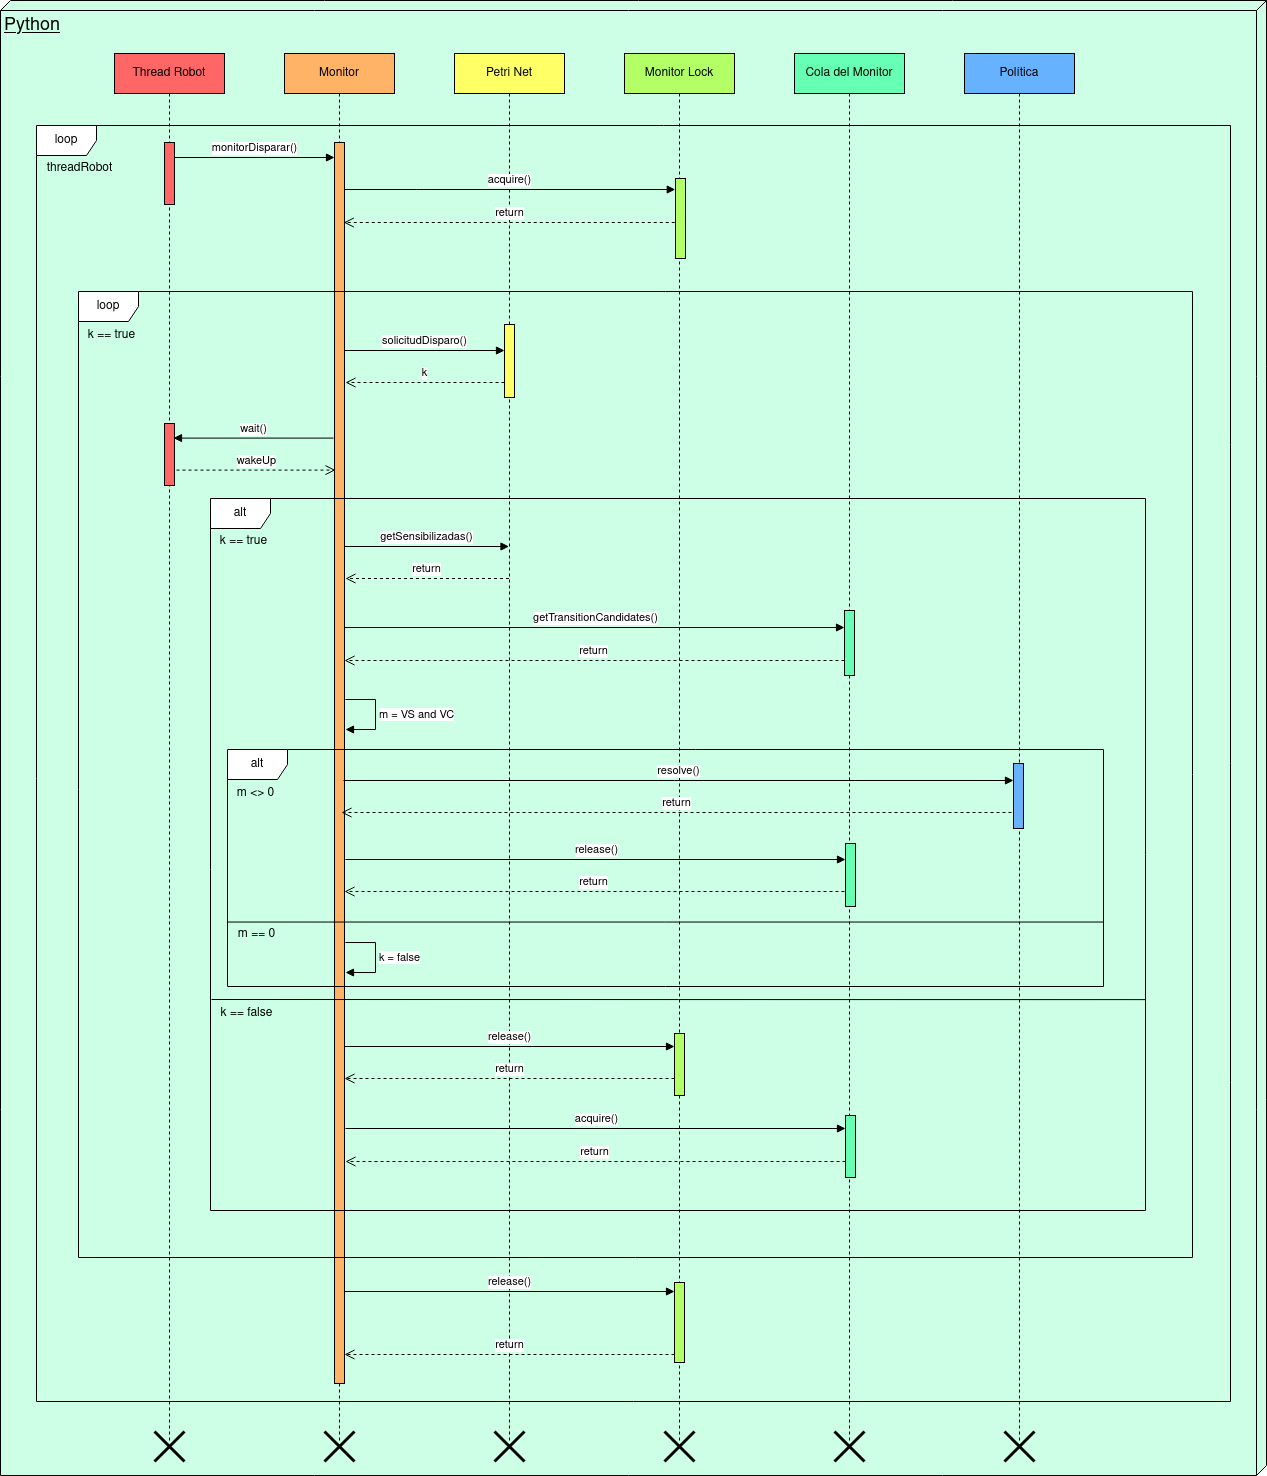
\includegraphics[width=1.0\linewidth]{images/diagrama_monitor.drawio.png}
    \caption{Diagrama de secuencia del monitor}
    \label{fig:diagrama_monitor}
\end{figure}